\documentclass[twocolumn]{aastex62}
\emergencystretch=1.em
\newcommand \figPath{./}
\newcommand \redColor{\color{red}}
\newcommand{\vecb}[1]{{#1}}
\renewcommand\labelenumi{(\roman{enumi})}
\renewcommand\theenumi\labelenumi
%\newcommand{\jcap}{JCAP}

\usepackage{amsmath,amsthm,amsfonts,amssymb,bm}
\usepackage{listings}
\usepackage{multirow}
\usepackage{color}

%\usepackage{subfigure}
\usepackage{textcomp}
\usepackage{epstopdf}
\usepackage{natbib}
\usepackage{commath}
\hypersetup{breaklinks}
\DeclareMathOperator{\arccosh}{arccosh}

\begin{document}
\title{Sparsity Weak Lensing Mass Reconstruction}
%\author{Xiangchong Li}
%\affiliation{Department of Physics, University of Tokyo, Tokyo 113-0033, Japan}
%\affiliation{Kavli Institute for the Physics and Mathematics of the Universe (WPI),\\
%University of Tokyo, Kashiwa 277-8583, Japan}
%\author{Masamune Oguri}
%\affiliation{Department of Physics, University of Tokyo, Tokyo 113-0033, Japan}
%\affiliation{Kavli Institute for the Physics and Mathematics of the Universe (WPI),\\
%University of Tokyo, Kashiwa 277-8583, Japan}
%\affiliation{Research Center for the Early Universe, University of Tokyo, Tokyo 113-0033, Japan}
%\author{Nobuhiko Katayama}
%\affiliation{Kavli Institute for the Physics and Mathematics of the Universe (WPI),\\
%University of Tokyo, Kashiwa 277-8583, Japan}
%\author{Wentao Luo}
%\affiliation{Kavli Institute for the Physics and Mathematics of the Universe (WPI),\\
%University of Tokyo, Kashiwa 277-8583, Japan}
%\author{Wenting Wang}
%\affiliation{Kavli Institute for the Physics and Mathematics of the Universe (WPI),\\
%University of Tokyo, Kashiwa 277-8583, Japan}
%\author{Jiaxin Han}
%\affiliation{Department of Astronomy, School of Physics and Astronomy, Shanghai Jiao Tong University, Shanghai, 200240, China}
%\affiliation{Kavli Institute for the Physics and Mathematics of the Universe (WPI),\\
%University of Tokyo, Kashiwa 277-8583, Japan}
%\author{HSC Collaboration}
%\noaffiliation
%\email{xiangchong.li@ipmu.jp}




\begin{abstract}

\end{abstract}

\section{Introduction}
Light from distant galaxies is lensed by the foreground inhomogeneous density distribution along the line-of-sight 
due to the influence of gravity and the shapes of the foreground galaxies are distorted due to the lensing effect. 
Such effect, which is known as weak lensing, imprints the information of foreground density distribution to the 
background galaxies and offers a direct probe into the mass density distribution in the universe. 

This paper is organized as follows. 
Section \ref{sec:MethodAll} proposes the new method for $3$-D mass map reconstruction. 
Section \ref{sec:Sim} introduces the realistic simulations we use to test the new method.
Section \ref{sec:Res} presents the results of our method on the simulations.
Section \ref{sec:Sum} summarizes and discusses the future development of the method.

\section{Methodology}
\label{sec:MethodAll}

\subsection{The Problem}
\subsubsection{Density Contrast to Shear}
We first review how the foreground density contrast induces the shear distortion on background galaxies.
The lensing distortion $\kappa$ at a comoving distance $\chi_s$ caused by the foreground inhomogeneous 
density distribution at a comoving distance $\chi_l$ ($\chi_l< \chi_s$) is

\begin{figure*}
    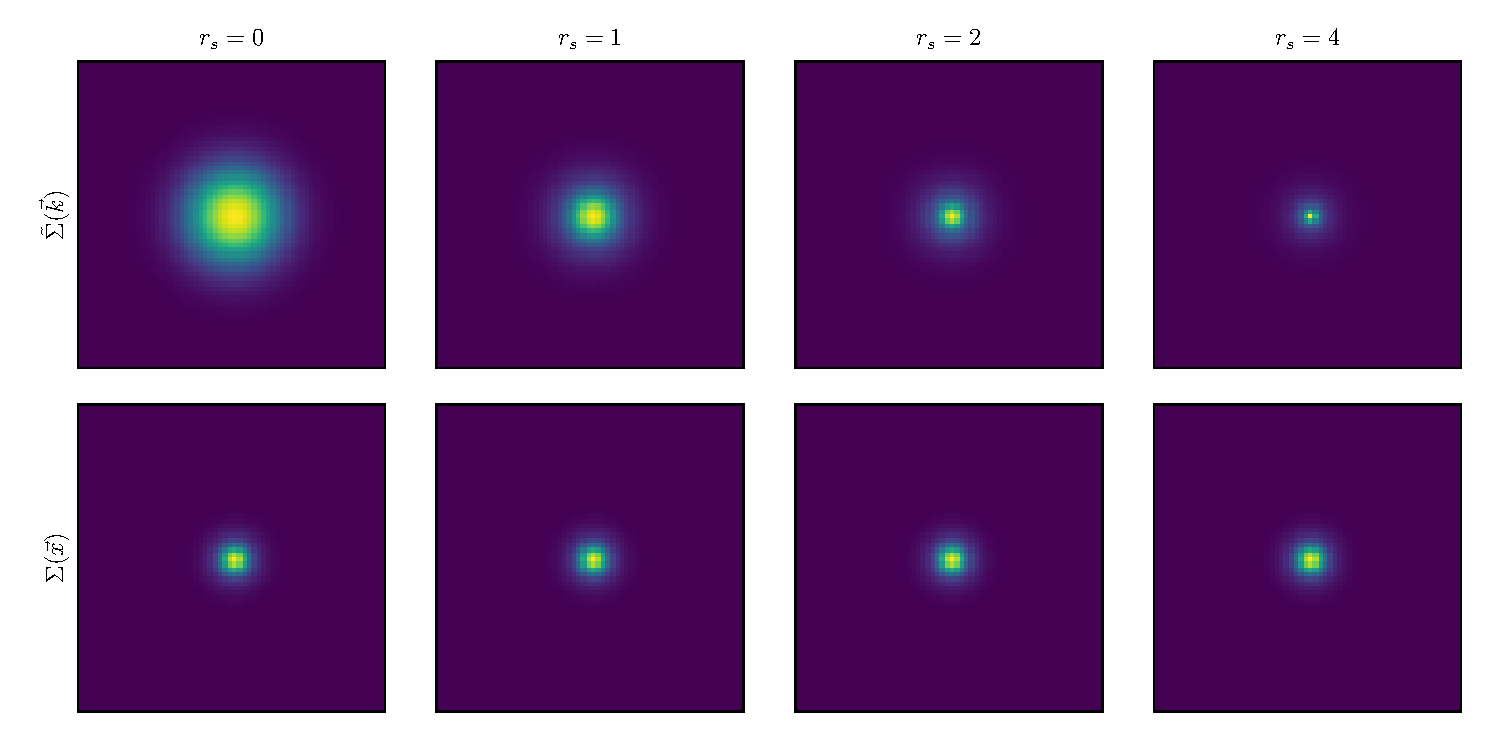
\includegraphics[width=0.95\textwidth]{nfwlet-atom-2D.pdf}
    \caption{The NFW atom with different scale radius ($r_s$). The first row shows the NFW atoms in Fourier 
            space and the second row shows the NFW atom in Real space.}
\end{figure*}


\begin{equation}
\kappa(\vec{\theta},\chi_s)=\frac{3H_0^2\Omega_M}{2 c^2} \int_0^{\chi_s} d\chi_l \frac{\chi_l \chi_{sl}}{\chi_s}
\frac{\delta(\vec{\theta},\chi_l)}{a(\chi_l)},
\end{equation}
\citep{massMap-Glimpse3D2014}.
where $\chi$ refers to the comoving distance, $\delta=\rho(\vec{\theta},\chi_l)/\bar{\rho}-1$ is the density contrast
at the position of lens, $H_0$ is the Hubble parameter, $\Omega_M$ is the matter density parameter, $c$ is the speed 
of light, and $a(\chi_l)$ is the scale parameter at the lens position. 

Substitute comoving distance ($\chi$) with redshift ($z$)
$z$ and we have
\begin{equation}\label{eq-delta2kappa}
\kappa(\vec{\theta},z_s)=\int_0^{z_s} dz_l \delta_{c}^{-1}(z_l,z_s)\delta(\vec{\theta},z_l).
\end{equation}
We term $\delta_{c}(z_l,z_s)$ as lensing critical density contrast and define it as
\begin{equation}
\delta_{c}^{-1}(z_l,z_s) =
\begin{cases}
\frac{3H_0\Omega_M}{2 c} \frac{\chi_l \chi_{sl} (1+z_l)}{\chi_{s} E\left(z_l\right)} & (z_s>z_l),\\
0&(z_s \leq z_l).
\end{cases}
\end{equation}

As shown in \citet{massMap-KS1993}, the shear distortion is related to the kappa field at the redshift plane as
\begin{equation}\label{eq-kappa2gamma}
\vecb{\gamma}(\vec{\theta},z_s) = \int \vecb{D}(\vec{\theta}-\vec{\theta'}) \kappa(\vec{\theta'},z_s) d^2 \theta,
\end{equation}
where
\begin{equation}
\begin{split}
\vecb{D}(\vec{\theta})&=-\frac{1}{\pi}(\theta_1-i\theta_2)^{-2},\\
\vecb{\gamma}(\vec{\theta})&=\gamma_1(\vec{\theta})+i\gamma_2(\vec{\theta}).
\end{split}
\end{equation}

Combine equation (\ref{eq-delta2kappa}) with equation (\ref{eq-kappa2gamma}) and we have
\begin{equation}\label{eq-delta2gamma-z}
\vecb{\gamma}(\vec{\theta},z_s) = \int_0^{z_s} dz_l \frac{\delta_c(z_l,+\infty)}{\delta_{c}(z_l,z_s)} \int d^2 \theta'  \vecb{D}(\vec{\theta}-\vec{\theta'}) \frac{\delta(\vec{\theta'},z_l)}{\delta_c(z_l,+\infty)}.
\end{equation}

\subsubsection{Photo-$z$ Uncertainty}
\begin{figure}
 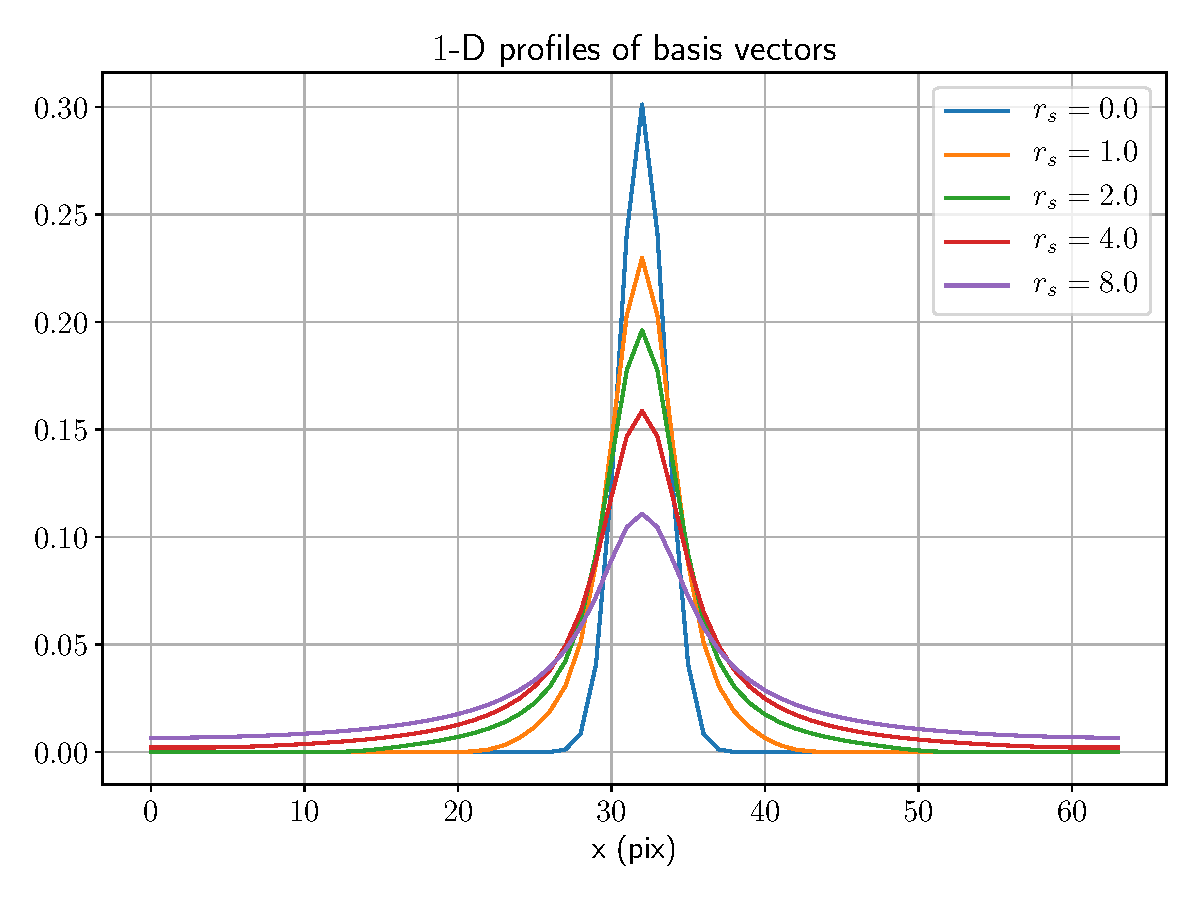
\includegraphics[width=0.5\textwidth]{nfwlet-atom-1D.pdf}
 \caption{The $1$-D slices of NFW atoms with different scale radius ($r_s=0,1,2,4,8$).}
\end{figure}
Since the redshifts of source galaxies in the current large scale survey are estimated with a limited 
number of photometric bands, the estimated redshift of a single galaxy suffers from large uncertainty. 
We denote the probability of a galaxies, with photo-$z$ estimated as $z_s$, being  located at redshift 
$z$ as $\mathcal{P}(z|z_s)$.  Note that, in order to simplify the future calculation, we assume the 
variation of the PDF across the transverse plane is small and neglect such variation.

Taking the uncertainty of redshift into account, equation (\ref{eq-delta2gamma-z}) changes to
\begin{equation}\label{eq-delta2gamma-poz}
\begin{split}
\gamma(\vec{\theta},z_s) &= \int_0^{z_s} dz_l P(z_l,z_s)\gamma(\vec{\theta},z_l,+\infty),\\
\gamma(\vec{\theta},z_l,+\infty)&= \int d^2 \theta'   Q(\vec{\theta}-\vec{\theta'},z_l) \delta(\vec{\theta'},z_l),
\end{split}
\end{equation}
where $\gamma(\vec{\theta},z_l,+\infty)$ represents shear signal at infinite redshift ($z_s=+\infty$) caused by density contrast at $z_l$, and $P(z_l,z_s)$ is the convolution kernel along line-of-sight and $Q(\vec{\theta},\vec{\theta}',z_l)$ is the convolution kernel along on the transverse plane. These kernels are defined as
\begin{equation}
\begin{split}
P(z_l,z_s)&=\int \frac{\delta_c(z_l,+\infty)}{\delta_{c}(z_l,z)} \mathcal{P}(z|z_s) dz,\\
Q(\vec{\theta},\vec{\theta'},z_l)&=\frac{\vecb{D}(\vec{\theta}-\vec{\theta'})}{\delta_c(z_l,+\infty)}.
\end{split}
\end{equation}

\subsubsection{Smoothing}
Since the observed galaxies have random irregular (unequally-spaced) distribution, it is necessary to smooth the shear signal in the observation. The smoothing is expressed as follows
\begin{equation}
\gamma_S  (\vec{\theta},z)  = \frac{\sum_i  W(\vec{\theta}-\vec{{\theta}}_i,z-z_i) e_i}{\sum_i W(\vec{\theta}-\vec{{\theta}}_i,z-z_i) R_i},
\end{equation}
where $W(\vec{\theta},z)$ is a $3$-D smoothing kernel. $e_i$, $R_i$, $z_i$ and $\theta_i$ are the ellipticity, response, reshift, transverse position of the `$i$-th' galaxy.
$W(\vec{\theta},z)$ can be decomposed into a transverse component $W_T(\vec{\theta})$ and a line-of-sight component $W_\times(z)$
\begin{equation}
W(\vec{\theta},z)=W_T(\vec{\theta}) W_\times (z).
\end{equation}
In this paper, we set
\begin{equation}
\begin{split}
W_T(\vec{\theta}) &=\frac{1}{2\pi\beta^2}\exp(-\frac{|\vec{\theta}|}{2\beta^2}),\\
W_\times (z) &=
\begin{cases}
1/\Delta z& (|z|<\Delta z/2),\\
0& else.
\end{cases}
\end{split}
\end{equation}

With the assumption that the density of response $R$ and the density of galaxy number vary slowly on the smoothing scale, the smoothed shear is
\begin{equation}\label{eq-smooth-gamma}
\gamma_S(\vec{\theta}_j,z_j)= \int d^2 \theta_s d z_sW(\vec{\theta}_j-\vec{{\theta}}_s,z_j-z_s) \gamma(\vec{\theta}_s,z_s)
\end{equation}

Substitute equation (\ref{eq-delta2gamma-poz}) into equation (\ref{eq-smooth-gamma})
\begin{equation}\label{eq-delta2gamma-smooth}
\begin{split}
\gamma_S(\vec{\theta}_j,z_j) &= \int_0^{z_j} dz_l P_S(z_l,z_j)\gamma_S(\vec{\theta}_j,z_l,+\infty),\\
\gamma_S(\vec{\theta}_j,z_l,+\infty)&= \int d^2 \theta'   Q_S(\vec{\theta}_j,\vec{\theta'},z_l) \delta(\vec{\theta'},z_l),
\end{split}
\end{equation}
and
\begin{equation}
\begin{split}
P_S(z_l,z_j)&=\int  dz_s W_\times (z_j-z_s) \int \frac{\delta_c(z_l,+\infty)}{\delta_{c}(z_l,z)} \mathcal{P}(z|z_s) dz,\\
Q_S(\vec{\theta},\vec{\theta'},z_l)&=\int d^2\theta'' W_T( \vec{\theta} -\vec{\theta''} )  \frac{\vecb{D}(\vec{\theta''}-\vec{\theta'})}{\delta_c(z_l,+\infty)}.
\end{split}
\end{equation}


\subsubsection{Mask and Noise}
In real observations, the influence of mask and noise should also be taken into account. The final observed shear is
\begin{equation}\label{eq-delta2gamma-final}
\gamma_o(\vec{\theta},z)=M(\vec{\theta},z) \gamma(\vec{\theta},z) + \epsilon(\vec{\theta},z),
\end{equation}
where $\epsilon$ represents noise typically caused by random shape of intrinsic galaxies and such noise is modeled as white Gaussian noise. $M(\vec{\theta},z_s)$ is the mask function.

We can write equation (\ref{eq-delta2gamma-final}) into
\begin{equation}\label{eq-delta2gamma-operator-final}
\gamma_o =\mathbf{M}  \mathbf{P} \mathbf{Q} \delta + \epsilon,
\end{equation}
where $\mathbf{M}$,  $\mathbf{P}$ and $\mathbf{Q}$ represent the functional operators $M$, $P$ and $Q$, respectively.

\subsection{The Method}
\label{sec:kappaMap}

\subsubsection{Dictionary}
Since many $N$-body simulations have shown the dark matter to be largely distributed in halos connected by filaments,
we assume that the density contrast field can be decomposed into multi-scaled NFW halo \citep{halo-NFW1997ApJ} and point mass at different positions
\begin{equation}
\delta(\vec{x}) = \sum_{s=0}^{N_s} \int d^3 x' \phi_s(\vec{x}-\vec{x}') \alpha_s(\vec{x'})\\
\end{equation}
where $\phi_0$ is $3$-D Dirac delta function representing point mass
\begin{equation}
\phi_0(\vec{x})= \delta_D(\theta_1) \delta_D(\theta_2) \delta_D(z).
\end{equation}
Since the scale of halo is much less than the reachable redshift resolution, we neglect the depth of halo on the line-of-sight direction as suggested by \citep{massMap-Glimpse3D2014}.
On the transverse plane, the NFW atom is modeled with the surface density profile of NFW halo with scale $\theta_s$ and truncation radius $c \theta_s$ \citep{haloModel-TJ2003-3pt}, where $c$ is generally known as concentration of NFW halo.  Whereas, the NFW atom is modeled with Dirac delta function on the line-of-sight direction


\begin{equation}
\begin{split}
\phi_s(\vec{x}) =&\frac{f }{2 \pi \theta_s^2 } F(|\vec{\theta}|/\theta_s) \delta_D(z),\\
&  (s=1..N_s)
\end{split}
\end{equation}
where
\begin{equation}
F(x)=
\begin{cases}
-\frac{\sqrt{c^2-x^2}}{(1-x^2)(1+c)} + \frac{\arccosh \left(\frac{x^2+c}{x(1+c)}\right)}{(1-x^2)^{3/2}}  & (x<1),\\
\frac{\sqrt{c^2-1}}{3(1+c)} (1+\frac{1}{c+1}) & (x=1),\\
-\frac{\sqrt{c^2-x^2}}{(1-x^2)(1+c)} + \frac{\arccos\left(\frac{x^2+c}{x(1+c)}\right)}{(x^2-1)^{3/2}} & (1<x\leq c),\\
0& (x>c).
\end{cases}
\end{equation}
and $f=1/[\ln (1+c)-c/(1+c)]$.

$\alpha_s$ is the corresponding decomposition coefficient of the density contrast field onto our basis atom. The total coefficients set is denoted as $\alpha=\begin{pmatrix}
\alpha_0\\
\alpha_1\\
...\\
\alpha_{N_s}
\end{pmatrix}$, and the total dictionary is $\Phi=\begin{pmatrix}
\phi_0, \phi_1, ..., \phi_{N_s}
\end{pmatrix}$.

We pixelize the parameter space into a $N_\theta \times N_\theta \times N_l$ grid. $N_\theta$ is the number of pixels on the two dimensions of the transverse plane and $N_l$ is the number of pixels on the line-of-sight direction for the lenses. Similarly, $\gamma_o$ is pixelized onto a $N_\theta \times N_\theta \times N_s$ grid, where $N_s$ is the number of pixel on the line-of-sight direction for the sources.
The pixel size for the two dimensions on the transverse plane is denoted as $\Delta \theta$ and the pixel size for the line-of-sight direction is denoted as $\Delta z$.
Equation (\ref{eq-delta2gamma-operator-final}) changes to
\begin{equation}\label{eq-alpha2gamma-operator}
\gamma=\mathbf{M}\mathbf{P}\mathbf{Q}\mathbf{\Phi} \alpha +\epsilon.
\end{equation}

\subsubsection{Loss Function with Constrains}
\begin{figure}
 \centering
 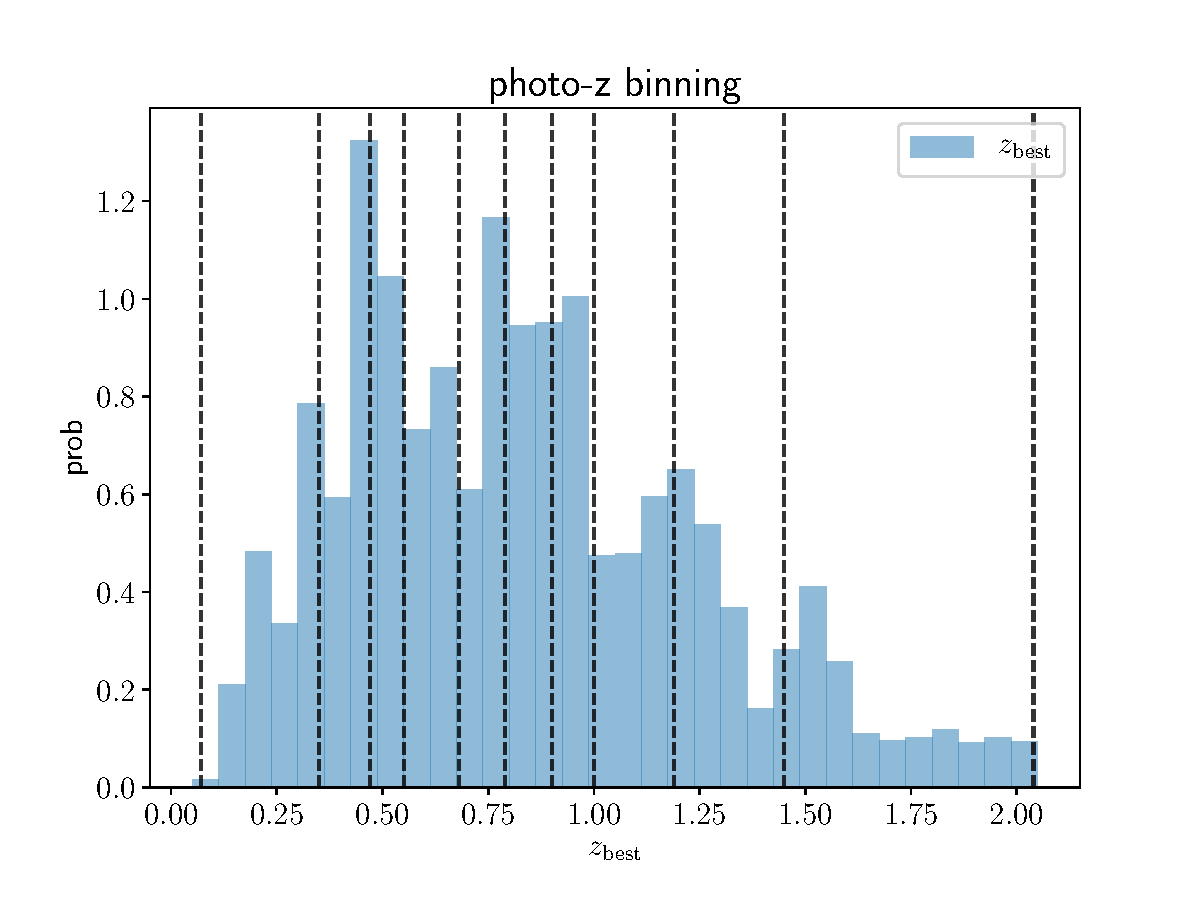
\includegraphics[width=0.5\textwidth]{photo-z_binning.pdf}
 \caption{The source galaxies are binned into $10$ redshift bins according to their mlz best photo-$z$ estimation. The blue histogram is the number distribution of the best photo-$z$ estimation. The vertical dashed lines are the bounds of bins. The galaxies are evenly distributed in each bins.}
\end{figure}

The loss function is defined as
\begin{equation}\label{eq-lossFun}
L = \norm{\gamma-\mathbf{M}\mathbf{P}\mathbf{Q}\mathbf{\Phi} \alpha}^2_2+\lambda \norm{\alpha}^1_1 + \tau\mathrm{TSV}(\alpha_0),
\end{equation}
where $\norm{\gamma-\mathbf{M}\mathbf{P}\mathbf{Q}\mathbf{\Phi} \alpha}^2_2$ is the normal chi-square, $\norm{\alpha^{N,P}}^1_1$ is the sparsity constrain, and $\mathrm{TSV}(\alpha^P)$ is the Total Squared Variation (TSV) constrain. $\norm{\bullet}_1$ and $\norm{\bullet}_2$ represent $l_1$ norm and $l_2$ norm, respectively.
The $\mathrm{TSV}$ operator is defined as
\begin{equation}
\begin{split}
\mathrm{TSV}(\alpha_0) =&  \sum_{ijk} \{ (\alpha_0[i,j,k]-\alpha_0[i+1,j,k])^2\\
&+(\alpha_0[i,j,k]-\alpha_0[i,j+1,k])^2\\
&+(\alpha_0[i,j,k]-\alpha_0[i,j,k+1])^2 \},
\end{split}
\end{equation}
where $i=1..N_\theta$, $j=1..N_\theta$, are the pixel indexes for the two dimensions on the transverse plane, $k=1..N_l$ is the pixel index on the line-of-sight direction.

\begin{figure}
 \centering
 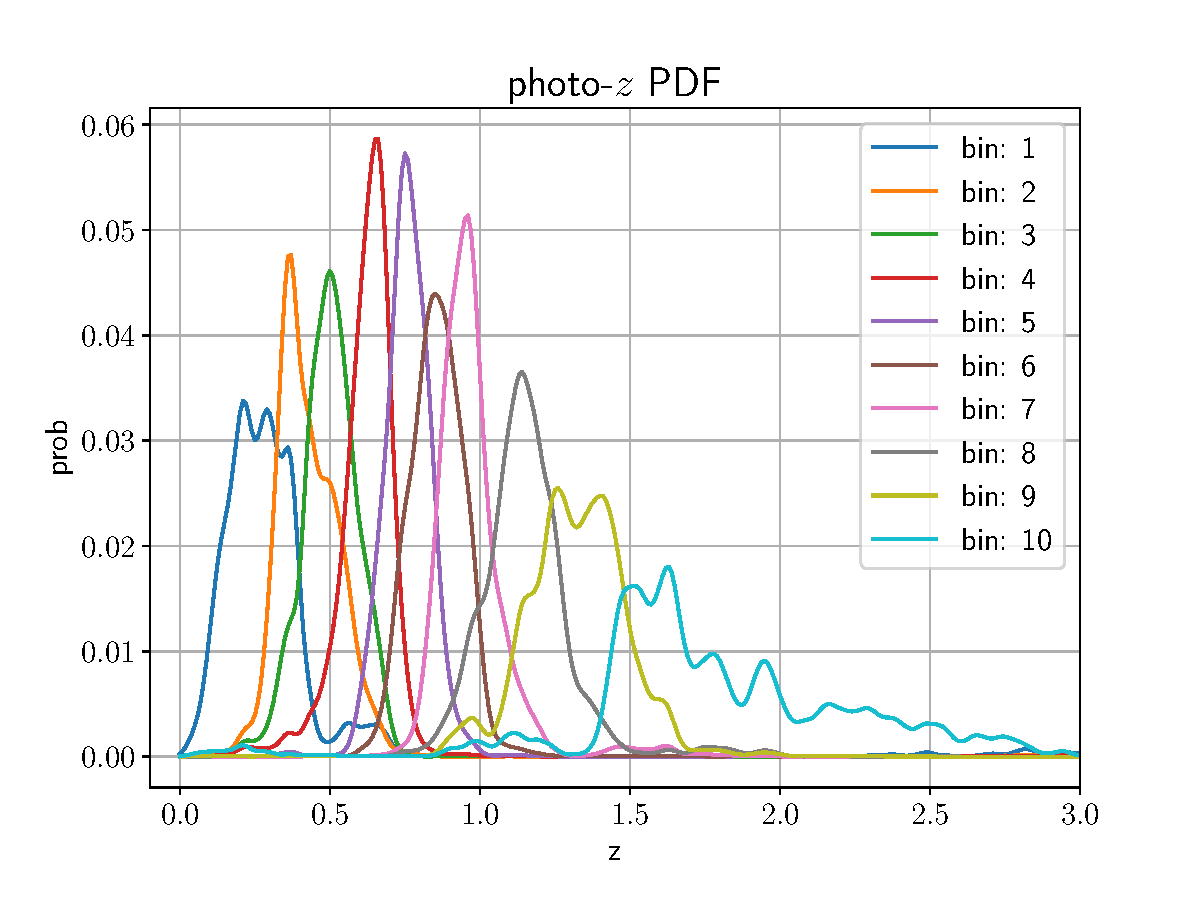
\includegraphics[width=0.5\textwidth]{mlz-poz.pdf}
 \caption{The PDF of photo-$z$ error for $10$ source redshift bins.}
\end{figure}

We define
\begin{equation}
\begin{split}
f(\alpha) &= \norm{\gamma-\mathbf{M}\mathbf{P}\mathbf{Q}\mathbf{\Phi} \alpha}^2_2+ \tau\mathrm{TSV}(\alpha^P)\\
&= \sum_{lm} A_{lm} \alpha_l \alpha_m + \sum_{l}B_{l} \alpha_l +C,
\end{split}
\end{equation}
where $l,m$ go over the indexes of $(i,j,k,s)$.


\begin{figure}
 \centering
 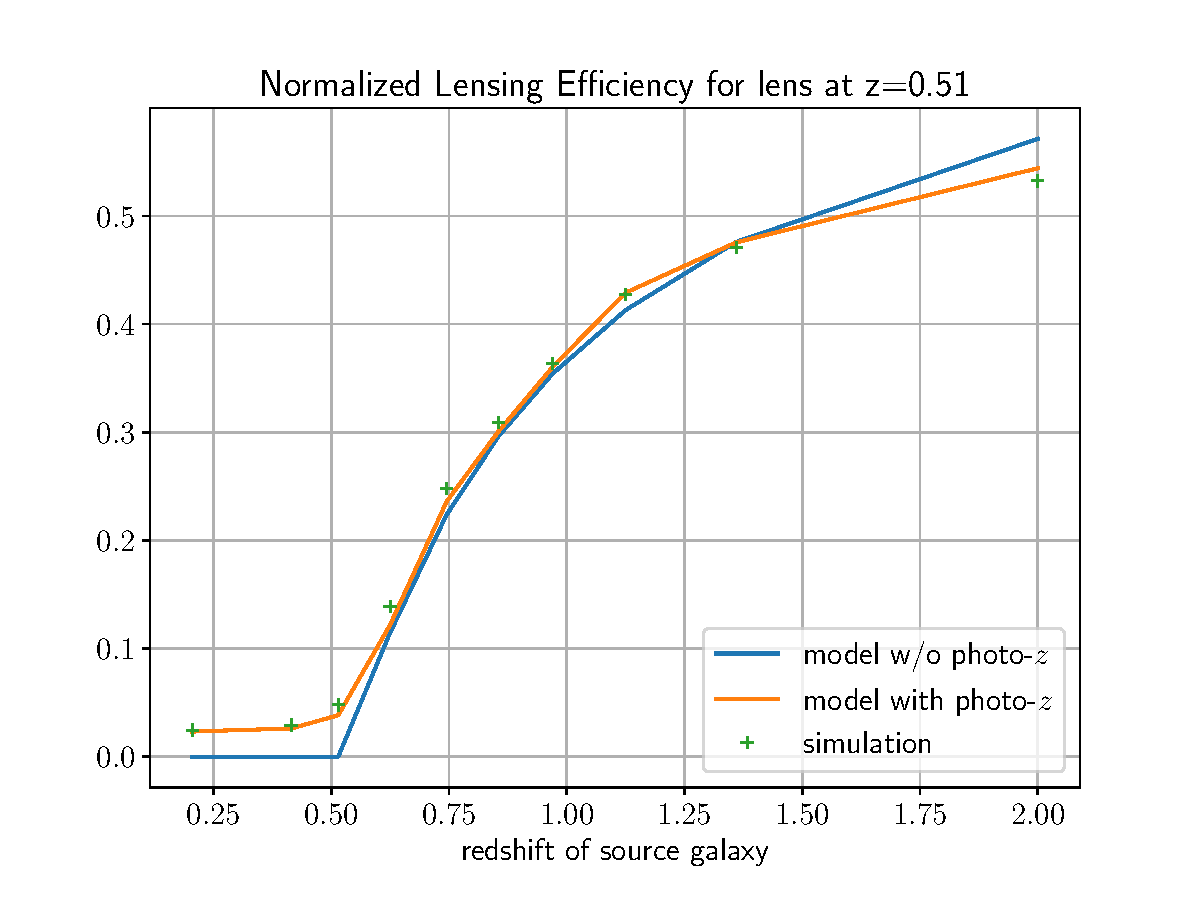
\includegraphics[width=0.5\textwidth]{lensing_efficiency.pdf}
 \caption{The blue line shows the normalized lensing efficiency for lens bin at $z_{l}=0.51$. 
 The orange line is the normalized lensing efficiency while taking into account the photo-$z$ uncertainty. 
 The green data points show the averaged $\kappa$ field for different redshift bins in the simulation.}
\end{figure}


\subsubsection{FISTA}
The basic FISTA algorithms is
\begin{equation}
X^{(n+1)}_m=\mathrm{ST}_{\lambda} (\alpha_m -\frac{\mu}{2A_{mm}} \frac{\partial f}{\partial \alpha_m})|_{\alpha^{(n)}_m} ,
\end{equation}
where
\begin{equation}
\mathrm{ST}_{\lambda} (x) = \mathrm{sign} (x) \max (\abs{x}-\lambda,0)
\end{equation}
is the soft thresholding function.

\begin{equation}
\begin{split}
t^{(n+1)} &= \frac{1+\sqrt{1+4(t^{(n)})^2}}{2},\\
\alpha^{(n+1)}_m& = X^{(n+1)}_m+[\frac{t^{(n)}-1}{t^{(n+1)}}(X^{(n+1)}_m-X^{(n)}_m)].
\end{split}
\end{equation}
The iteration is initialized with $t^{(0)}=1$ and $X^{(0)}=\alpha^{(0)}$.

\section{Simulation}
\label{sec:Sim}
This section simulates lensing shear fields induced by a group of dark matter halos with various halo mass and redshifts.
HSC-like shape measurement error and photo-$z$ error are added to the shear field.

\subsection{Weak Lensing Fields}

We simulate weak lensing shear fields of NFW halos according to \citet{haloModel-TJ2003-3pt} 
and sample halos in the mass-redshift plane as shown in Figure \ref{fig:mass-redshift}.
We assume a dependency of the concentration on the mass and the redshift of a halo 
\begin{equation}
c_{h}=6.02\times(\frac{M_{200}}{10^{13} M_{\odot}})^{-0.12}(\frac{1.47}{1.+z_h})^{0.16}.
\end{equation}


\begin{figure}[!ht]
 \centering
 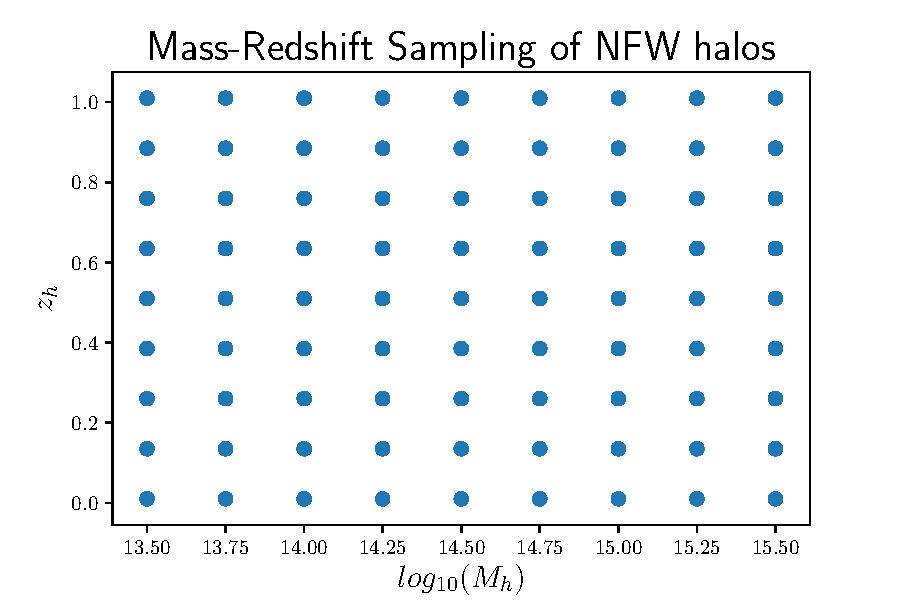
\includegraphics[width=0.45\textwidth]{mass-redshift-sampling.pdf}
 \caption{The sampling points of halos in the mass-redshift plane.}
 \label{fig:mass-redshift}
\end{figure}

\subsection{HSC-like Errors}
\subsubsection{Shear Measurement Error}
\begin{figure}[!ht]
 \centering
 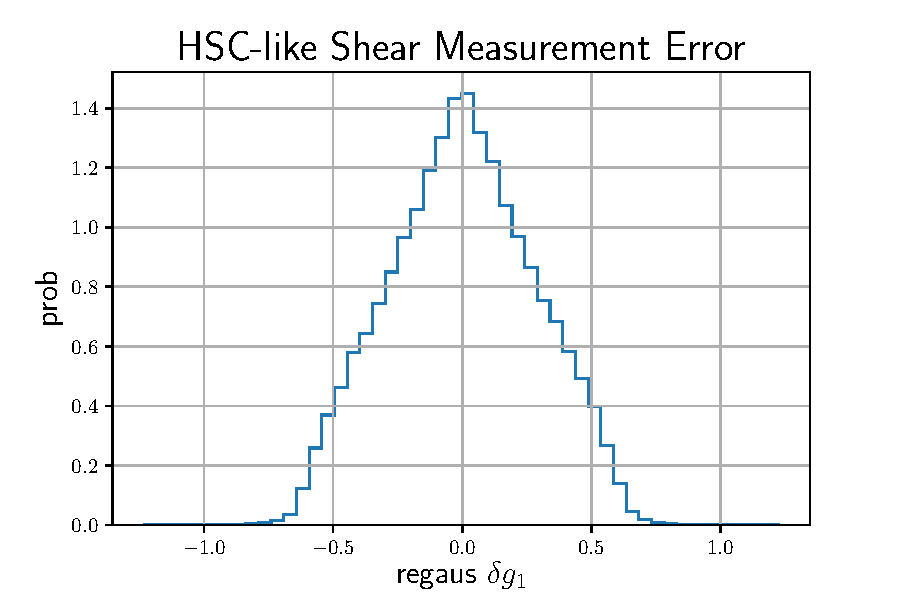
\includegraphics[width=0.45\textwidth]{shapeMeasurementError-HSCY1.pdf}
 \caption{HSC-like measurement error on the first component of shear ($g_1$).}
 \label{fig:mass-redshift}
\end{figure}

\subsubsection{Photo-$z$ Error} 

\section{Results}
\label{sec:Res}

\subsection{Detection Rate}

\subsection{Mass and Redshift Estimation}


\section{Summary}
\label{sec:Sum}

\begin{figure}[!ht]
 \centering
 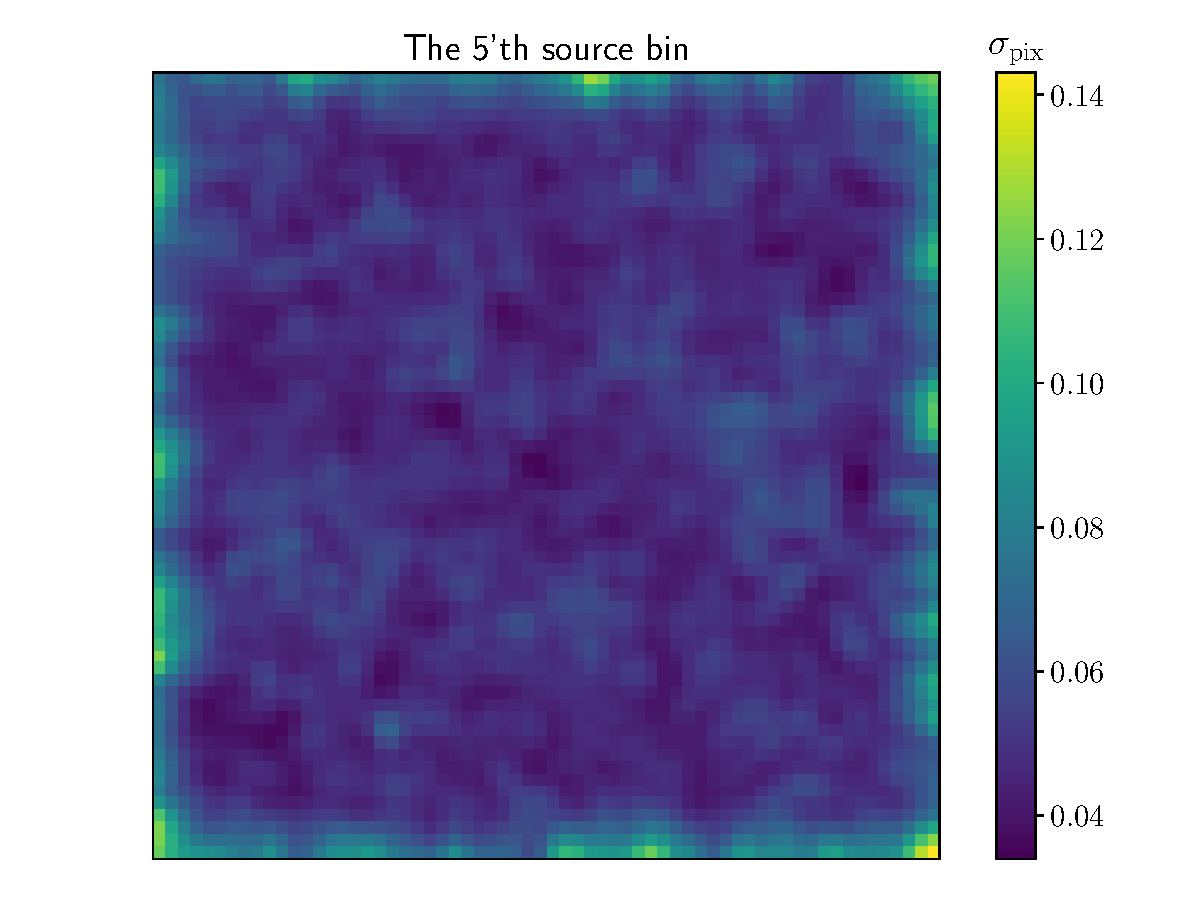
\includegraphics[width=0.45\textwidth]{noise_std_map_pix.pdf}
 \caption{The standard deviation map of shear measurement error for the fifth source bin ($0.69 \leq z < 0.80 $).}
\end{figure}

\bibliographystyle{aasjournal}
\bibliography{weak_lensing,lensCat,cosmoSim,cmbObs,gglens,shearCor,massMap,other}

\appendix
\section{General linear LASSO}
Note that the loss function defined in equation (\ref{eq-lossFun}) into
\begin{equation}
L(\alpha)=f(\alpha) +\lambda \norm{\alpha}^1_1,
\end{equation}
where
\begin{equation}
f(\vec{\alpha}) = \vec{\alpha}^T \mathbf{A} \vec{\alpha} + \vec{B} \cdot \vec{\alpha} +C.
\end{equation}
Using Einstein notation, we have
\begin{equation}
L(\alpha_i) = A_{ij} \alpha_i \alpha_j + B_{i} \alpha_i + C +\lambda_i \abs{\alpha_i}.
\end{equation}
Set the initial parameter vector is $\vec{\alpha}^{(0)}$. We focus on one specific parameter with index $\mu$ and fix other parameters with indexes $i \neq \mu$
\begin{equation}
L(\alpha_\mu| \alpha^{(0)}_{i\neq\mu})=A_{\mu\mu} \alpha_\mu^2 + (A_{i\mu}\alpha^{(0)}_i+A_{\mu i}\alpha^{(0)}_i +B_\mu) \alpha_\mu +\lambda_\mu \abs{\alpha_\mu} +B_i \alpha^{(0)}_i + \lambda_i \abs{\alpha^{(0)}_i} +C
\end{equation}
reach its minimum at $\mathrm{ST}_{\lambda} (\alpha_\mu -\frac{\partial_\mu f(\alpha_\mu| \alpha^{(0)}_{i\neq\mu})}{2A_{\mu\mu}}) |_{\alpha_\mu^{(0)}}$,
where $\mathrm{ST}_{\lambda} (x) = \mathrm{sign} (x) \max (\abs{x}-\lambda,0)$ is the soft thresholding function. Then the parameter can be updated
\begin{equation}
\alpha^{(1)}_\mu \leftarrow \mathrm{ST}_{\lambda} (\alpha_\mu -\frac{\partial_\mu f(\alpha_\mu| \alpha^{(0)}_{i\neq\mu})}{2A_{\mu\mu}}) |_{\alpha_\mu^{(0)}}.
\end{equation}
Other parameters are subsequently updated in the same way. The minimum of the loss function can be reached by iterating the parameter update.

\end{document}
